% =====================================================================
%  Лабораторная работа №4. Численное интегрирование.
%  Вариант 4: integral from 2.2 to 3.4 of x^2/(x^2+1) dx.
%
%  Сборка (любой из вариантов):
%      pdflatex  BastrakovReport.tex
%      xelatex   BastrakovReport.tex
%      lualatex  BastrakovReport.tex
%  (запускать два раза — для оглавления и перекрёстных ссылок)
% =====================================================================
\documentclass[14pt,a4paper]{extarticle}

% - Поддержка кириллицы: pdfLaTeX (T2A) либо XeLaTeX/LuaLaTeX (fontspec) -
\usepackage{iftex}
\ifPDFTeX
    \usepackage[T2A]{fontenc}
    \usepackage[utf8]{inputenc}
    \usepackage[russian]{babel}
    \usepackage{tempora}
    \usepackage{listingsutf8}
\else
    \usepackage{fontspec}
    \usepackage{polyglossia}
    \setdefaultlanguage{russian}
    \setotherlanguage{english}
    \IfFontExistsTF{Liberation Serif}%
        {\setmainfont{Liberation Serif}}%
        {\IfFontExistsTF{PT Serif}%
            {\setmainfont{PT Serif}}%
            {\setmainfont{TeX Gyre Termes}}}
    \IfFontExistsTF{DejaVu Sans Mono}%
        {\setmonofont{DejaVu Sans Mono}}%
        {\IfFontExistsTF{Liberation Mono}%
            {\setmonofont{Liberation Mono}}%
            {\setmonofont{TeX Gyre Cursor}}}
\fi

% - Математика, графика, оформление -----------
\usepackage{amsmath,amssymb}
\usepackage{graphicx}
\usepackage{geometry}
\usepackage{booktabs}
\usepackage{array}
\usepackage{float}
\usepackage{caption}
\usepackage{indentfirst}
\usepackage{xcolor}
\usepackage[hidelinks]{hyperref}

\geometry{a4paper,left=3cm,right=1.5cm,top=2cm,bottom=2cm}
\graphicspath{{graphics/img/}}

\captionsetup{labelsep=endash,justification=centering}
\setlength{\parindent}{1.25cm}
\setlength{\emergencystretch}{3em}
\tolerance=2000
\renewcommand{\arraystretch}{1.15}
\renewcommand{\labelenumi}{\arabic{enumi})}

\begin{document}

% =====================================================================
%  Титульный лист
% =====================================================================
\begin{titlepage}
    \centering
    \large
    Министерство образования и науки РФ\\[0.3cm]
    Пермский национальный исследовательский политехнический университет\\[0.3cm]
    Электротехнический факультет\\[0.3cm]
    Кафедра "Информационные технологии и автоматизированные системы"

    \vspace{3.5cm}
    {\Large Информатика в приложении к отрасли}\\[0.4cm]
    {\Large\bfseries Лабораторная работа № 4}\\[0.6cm]

    Тема: "Численное интегрирование"\\[0.2cm]
    Вариант 4

    \vspace{4.5cm}
    \begin{flushleft}
        \large
        Выполнил: студент группы РИС-25-2б \hfill Бастраков Данил\\[0.5cm]
        Проверил: профессор кафедры ИТАС \hfill Шварц К.~Г.\\[0.5cm]
        Дата: \underline{\hspace{3cm}} \hfill Подпись: \underline{\hspace{4cm}}
    \end{flushleft}

    \vfill
    Пермь\\ 2026
\end{titlepage}

\tableofcontents
\newpage

% =====================================================================
\section{Постановка задачи}
% =====================================================================

\textbf{Цель работы} --- вычислить определённый интеграл с заданной
точностью $\varepsilon=10^{-5}$ несколькими квадратурными формулами,
реализовать алгоритмы в программе и сравнить их эффективность.

\begin{equation}
    I=\int\limits_{2,2}^{3,4}\frac{x^2}{x^2+1}\,dx .
    \label{eq:integral}
\end{equation}

Подынтегральная функция $f(x)=x^2/(x^2+1)$ непрерывна и дифференцируема
на отрезке $[2,2;\,3,4]$, поэтому все рассматриваемые квадратуры
применимы. Её первообразной является $F(x)=x-\operatorname{arctg}x$,
поэтому точное значение интеграла~\eqref{eq:integral}:
\begin{equation}
    I=(3,4-\operatorname{arctg}3,4)-(2,2-\operatorname{arctg}2,2)
      =1{,}059423948590 .
    \label{eq:exact}
\end{equation}

Программа читает параметры задачи из файла \texttt{input.txt}: пределы
интегрирования $a$ и $b$, точность $\varepsilon$ и начальное число
частей $n_0$. Вид функции фиксирован вариантом~4, как и метод
в лабораторной работе №~3 был фиксирован видом сплайна.

% =====================================================================
\section{Краткое описание методов}
% =====================================================================

Пусть отрезок $[a,b]$ разбит на $n$ равных частей с шагом
$h=(b-a)/n$, $x_i=a+ih$, $y_i=f(x_i)$.

\subsection{Формула трапеций}

Формула трапеций имеет вид
\begin{equation}
    I_n=h\left(\frac{y_0}{2}+y_1+y_2+\ldots+y_{n-1}+\frac{y_n}{2}\right),
    \label{eq:trapezoid}
\end{equation}
а её остаточный член:
\begin{equation}
    R_n(f)=-\frac{(b-a)^3}{12n^2}f''(\xi),\qquad a\le \xi\le b .
    \label{eq:trapezoid-error}
\end{equation}

\textbf{Геометрическая интерпретация.} Отрезок $[x_i,x_{i+1}]$ заменяется
трапецией с основаниями $y_i$ и $y_{i+1}$ и высотой $h$; площадь этой
трапеции равна $h(y_i+y_{i+1})/2$. Сумма площадей всех трапеций и даёт
приближение~\eqref{eq:trapezoid}. Формула точна для многочленов первой
степени, а порядок её погрешности --- $O(h_s^2)$.

\subsection{Формула Симпсона}

Для чётного $n$:
\begin{equation}
    I_n=\frac{h}{3}\left[y_0+y_n
       +2(y_2+y_4+\ldots+y_{n-2})
       +4(y_1+y_3+\ldots+y_{n-1})\right],
    \label{eq:simpson}
\end{equation}
\begin{equation}
    R_n(f)=-\frac{(b-a)^5}{180n^4}f^{(IV)}(\xi),\qquad a\le \xi\le b .
    \label{eq:simpson-error}
\end{equation}

\textbf{Геометрическая интерпретация.} Каждые два соседних отрезка
объединяются, и через три соответствующие точки кривой проводится
парабола; интеграл аппроксимируется площадью под этой параболой.
Поэтому число частей разбиения $n$ обязательно должно быть чётным:
$[a,b]$ должен разбиваться на пары отрезков, на каждую из которых
приходится одна парабола по трём узлам. Формула Симпсона точна для
многочленов до третьей степени включительно, её порядок --- $O(h^4)$.

\subsection{Формула Гаусса--Лежандра}

Обычная квадратура Гаусса (Гаусса--Лежандра) с весом $p(x)=1$
на отрезке $[a,b]$ использует неравномерные узлы и веса:
\begin{equation}
    I\approx\frac{b-a}{2}\sum_{i=1}^{n}C_i f(x_i),\qquad
    x_i=\frac{a+b}{2}+\frac{b-a}{2}t_i .
    \label{eq:gauss}
\end{equation}
Здесь $t_i$ --- нули многочлена Лежандра $P_n$ на $[-1,1]$, а $C_i$ ---
соответствующие веса. Значения $t_i$ и $C_i$ берутся из таблицы
квадратурных коэффициентов Гаусса--Лежандра. Для $n=4$ и $n=5$
они приведены в табл.~\ref{tab:gauss-nodes}.

\textbf{Содержательная интерпретация.} В отличие от формул трапеций
и Симпсона, где узлы фиксированы заранее, в формуле Гаусса--Лежандра оптимально
выбираются и положения узлов $t_i$, и веса $C_i$. Это позволяет сделать
квадратуру точной для многочленов степени до $2n-1$ включительно,
то есть при том же числе вычислений функции получить более высокий
порядок точности.

\begin{table}[H]
    \centering
    \caption{Коэффициенты квадратуры Гаусса--Лежандра}
    \label{tab:gauss-nodes}
    \begin{tabular}{c|cc|cc}
        \toprule
        \multicolumn{3}{c|}{$n=4$} & \multicolumn{2}{c}{$n=5$}\\
        $t_i$ & $C_i$ & & $t_i$ & $C_i$\\
        \midrule
        $-0{,}861136$ & $0{,}347855$ & & $-0{,}906180$ & $0{,}236927$\\
        $-0{,}339981$ & $0{,}652145$ & & $-0{,}538469$ & $0{,}478629$\\
        $ 0{,}339981$ & $0{,}652145$ & & $ 0$          & $0{,}568889$\\
        $ 0{,}861136$ & $0{,}347855$ & & $ 0{,}538469$ & $0{,}478629$\\
        & & & $ 0{,}906180$ & $0{,}236927$\\
        \bottomrule
    \end{tabular}
\end{table}

\subsection{Правило Рунге}

Пусть $I_{n_1}$ и $I_{n_2}$ --- приближения по одной формуле при
$n_1$ и $n_2$ частях разбиения, а $m$ --- порядок остаточного члена.
Тогда уточнённое значение:
\begin{equation}
    I_{n_1,n_2}=I_{n_2}+\frac{n_1^m}{n_2^m-n_1^m}
                           \left(I_{n_2}-I_{n_1}\right).
    \label{eq:runge}
\end{equation}
При $n_2=2n_1$ получаем
\begin{equation}
    I_{n,2n}=I_{2n}+\frac{I_{2n}-I_n}{2^m-1},
    \label{eq:runge-double}
\end{equation}
причём для трапеций $m=2$ (знаменатель~3), а для Симпсона $m=4$
(знаменатель~15). В программе вычисление прекращается, как только
$|I_{2n}-I_n|<\varepsilon$; после этого результат уточняется по
формуле~\eqref{eq:runge-double}.

% =====================================================================
\section{Исходные данные}
% =====================================================================

Параметры задачи считываются из файла \texttt{input.txt};
\begin{center}
    \texttt{2.2\quad 3.4\quad 1e-5\quad 10}
\end{center}

\begin{table}[H]
    \centering
    \caption{Параметры расчёта}
    \label{tab:input}
    \begin{tabular}{c|c}
        \toprule
        Параметр & Значение\\
        \midrule
        $a$ & $2{,}2$\\
        $b$ & $3{,}4$\\
        $\varepsilon$ & $10^{-5}$\\
        $n_0$ & $10$\\
        \bottomrule
    \end{tabular}
\end{table}

% =====================================================================
\section{Результаты вычислений}
% =====================================================================

\subsection{Формула трапеций}

На каждом шаге число разбиений удваивалось: $n=10,20,40$ и~$80$.
Промежуточные результаты приведены в табл.~\ref{tab:trap}.

\begin{table}[H]
    \centering
    \caption{Уточнение по формуле трапеций ($m=2$)}
    \label{tab:trap}
    \small
    \begin{tabular}{crrrr}
        \toprule
        $n$ & $h$ & $I_n$ & $|I_{2n}-I_n|$ & $I_{n,2n}$\\
        \midrule
        10 & $0{,}12$ & $1{,}0593209017$ & $0{,}00007728$ & $1{,}0594239385$\\
        20 & $0{,}06$ & $1{,}0593981793$ & $0{,}00001933$ & $1{,}0594239480$\\
        40 & $0{,}03$ & $1{,}0594175058$ & $0{,}00000483$ & $1{,}0594239486$\\
        \bottomrule
    \end{tabular}
\end{table}

На последнем шаге $|I_{80}-I_{40}|=0{,}00000483<10^{-5}$, поэтому
вычисление завершено:
\begin{equation}
    I_{80}=1{,}059422337865,\qquad
    I_{40,80}=1{,}059423948551 .
\end{equation}

\subsection{Формула Симпсона}

Уже на первом шаге разность соседних приближений оказалась меньше
заданной точности (табл.~\ref{tab:simpson}).

\begin{table}[H]
    \centering
    \caption{Уточнение по формуле Симпсона ($m=4$)}
    \label{tab:simpson}
    \small
    \begin{tabular}{crrrr}
        \toprule
        $n$ & $h$ & $I_n$ & $|I_{2n}-I_n|$ & $I_{n,2n}$\\
        \midrule
        10 & $0{,}12$ & $1{,}0594237882$ & $0{,}00000015$ & $1{,}0594239486$\\
        \bottomrule
    \end{tabular}
\end{table}

\begin{equation}
    I_{20}=1{,}059423938542,\qquad
    I_{10,20}=1{,}059423948563 .
\end{equation}

\subsection{Формула Гаусса--Лежандра}

Для обоих вариантов $x_i=2{,}8+0{,}6\,t_i$. Вычисления сведены
в табл.~\ref{tab:gauss4} и~\ref{tab:gauss5}.

\begin{table}[H]
    \centering
    \caption{Квадратура Гаусса--Лежандра при $n=4$}
    \label{tab:gauss4}
    \small
    \begin{tabular}{crrrrr}
        \toprule
        $i$ & $C_i$ & $t_i$ & $x_i$ & $f(x_i)$ & $C_i f(x_i)$\\
        \midrule
        1 & $0{,}347855$ & $-0{,}861136$ & $2{,}283318$ & $0{,}839061$ & $0{,}291872$\\
        2 & $0{,}652145$ & $-0{,}339981$ & $2{,}596011$ & $0{,}870789$ & $0{,}567881$\\
        3 & $0{,}652145$ & $ 0{,}339981$ & $3{,}003989$ & $0{,}900239$ & $0{,}587086$\\
        4 & $0{,}347855$ & $ 0{,}861136$ & $3{,}316682$ & $0{,}916669$ & $0{,}318868$\\
        \midrule
        \multicolumn{5}{r}{$\sum C_i f(x_i)$} & $1{,}765706581$\\
        \bottomrule
    \end{tabular}
\end{table}

\begin{equation}
    I^{(4)}=0{,}6\cdot1{,}765706580935=1{,}059423948561 .
    \label{eq:gauss4-result}
\end{equation}

\begin{table}[H]
    \centering
    \caption{Квадратура Гаусса--Лежандра при $n=5$}
    \label{tab:gauss5}
    \small
    \begin{tabular}{crrrrr}
        \toprule
        $i$ & $C_i$ & $t_i$ & $x_i$ & $f(x_i)$ & $C_i f(x_i)$\\
        \midrule
        1 & $0{,}236927$ & $-0{,}906180$ & $2{,}256292$ & $0{,}835819$ & $0{,}198028$\\
        2 & $0{,}478629$ & $-0{,}538469$ & $2{,}476918$ & $0{,}859848$ & $0{,}411548$\\
        3 & $0{,}568889$ & $ 0$          & $2{,}800000$ & $0{,}886878$ & $0{,}504535$\\
        4 & $0{,}478629$ & $ 0{,}538469$ & $3{,}123082$ & $0{,}907008$ & $0{,}434120$\\
        5 & $0{,}236927$ & $ 0{,}906180$ & $3{,}343708$ & $0{,}917901$ & $0{,}217475$\\
        \midrule
        \multicolumn{5}{r}{$\sum C_i f(x_i)$} & $1{,}765706581$\\
        \bottomrule
    \end{tabular}
\end{table}

\begin{equation}
    I^{(5)}=0{,}6\cdot1{,}765706580994=1{,}059423948597 .
    \label{eq:gauss5-result}
\end{equation}

\subsection{Сравнение результатов}

Все методы дают значение, совпадающее с точным~\eqref{eq:exact}
в первых девяти знаках (табл.~\ref{tab:compare}).

\begin{table}[H]
    \centering
    \caption{Сравнение результатов}
    \label{tab:compare}
    \small
    \begin{tabular}{lrrr}
        \toprule
        Метод & $n$ (узлы) & $I$ & $|I-I_{\text{точн.}}|$\\
        \midrule
        Трапеции + Рунге & 80 & $1{,}059423948551$ & $3{,}93\cdot10^{-11}$\\
        Симпсон + Рунге  & 20 & $1{,}059423948563$ & $2{,}70\cdot10^{-11}$\\
        Гаусс--Лежандра, $n=4$ & 4  & $1{,}059423948561$ & $2{,}94\cdot10^{-11}$\\
        Гаусс--Лежандра, $n=5$ & 5  & $1{,}059423948597$ & $6{,}24\cdot10^{-12}$\\
        \bottomrule
    \end{tabular}
\end{table}

График подынтегральной функции, площадь под которой вычисляется,
и начальное разбиение на $n_0=10$ частей приведены
на рис.~\ref{fig:integral}.

\begin{figure}[H]
    \centering
    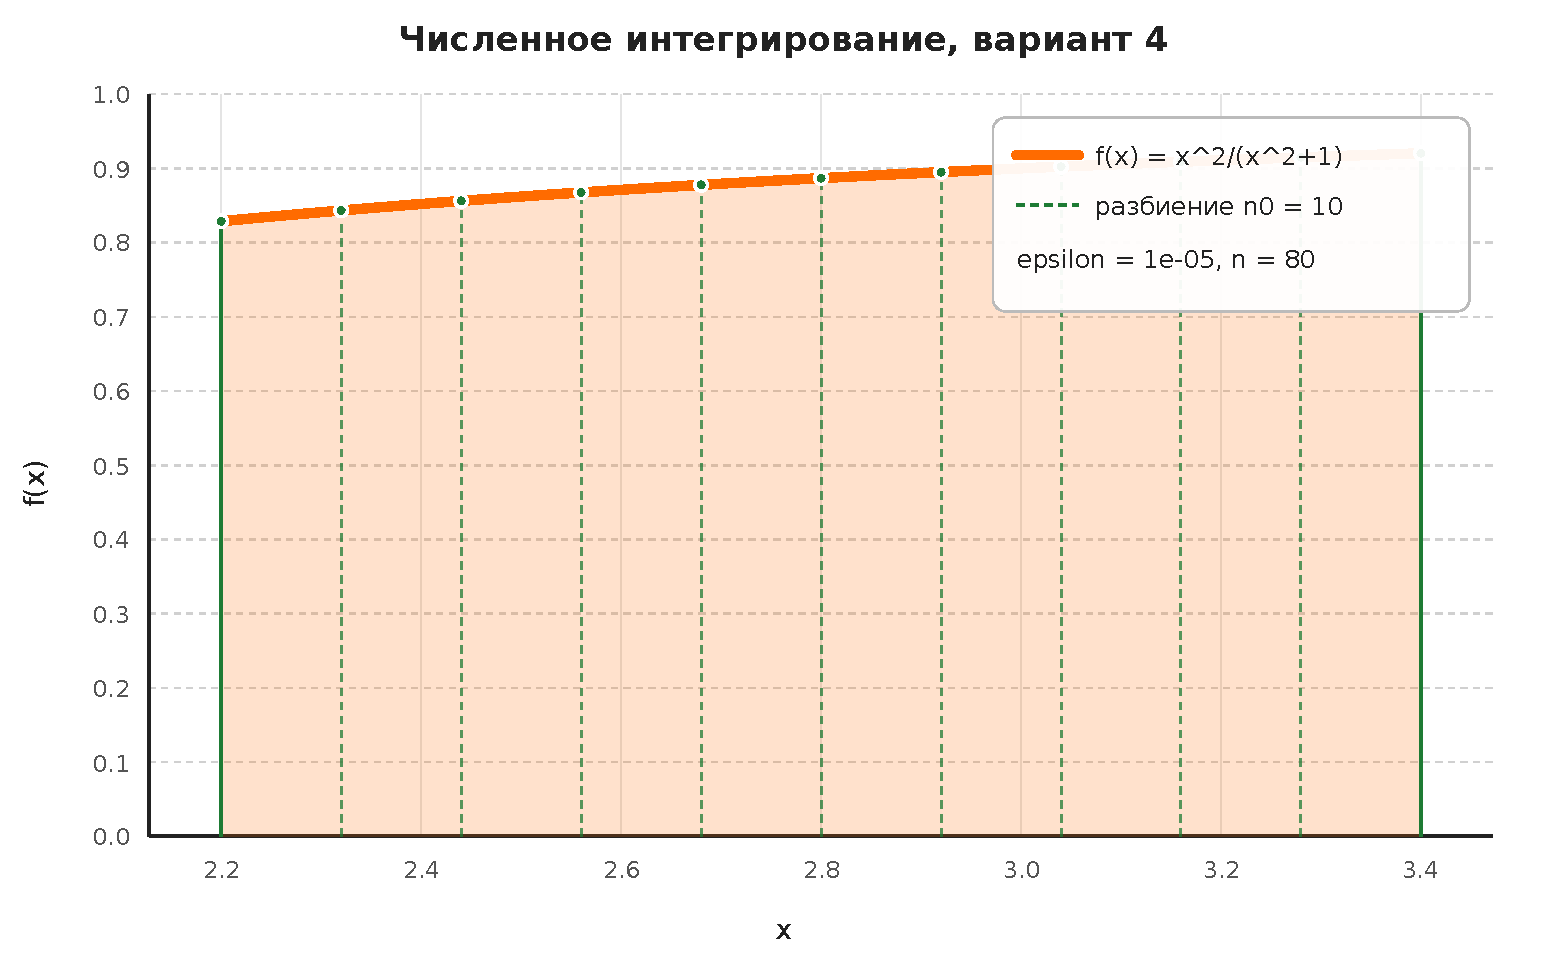
\includegraphics[width=0.9\textwidth]{fig_integral.pdf}
    \caption{Подынтегральная функция и область интегрирования, вариант~4}
    \label{fig:integral}
\end{figure}

% =====================================================================
\section{Обсуждение результатов}
% =====================================================================

Формула трапеций достигла критерия остановки $|I_{2n}-I_n|<10^{-5}$
только после трёх удвоений ($n=80$), в то время как формула
Симпсона --- уже после первого ($n=20$). Это согласуется с порядками
остаточных членов: $O(h^2)$ у трапеций и $O(h^4)$ у Симпсона.
После уточнения по Рунге обе формулы дают результат с погрешностью
порядка $10^{-11}$, то есть уточнение эффективно устраняет
ведущий член ошибки.

Квадратура Гаусса--Лежандра с четырьмя узлами по точности близка к уточнённой
формуле Симпсона, а с пятью узлами даёт наименьшую погрешность
($6{,}24\cdot10^{-12}$), используя всего пять значений функции.
Это подтверждает теоретическое свойство квадратур Гаусса--Лежандра:
при $n$ узлах они точны для многочленов степени $2n-1$, и для
гладкой функции $x^2/(x^2+1)$ на коротком отрезке такой порядок
оказывается достаточным для высокой точности.

Все расчёты выполнены программой на языке C\# с вводом данных
из файла \texttt{input.txt}; результаты выведены в виде таблиц,
что позволяет проследить каждое удвоение разбиения и каждый узел
квадратуры Гаусса--Лежандра.

\end{document}
